\documentclass[12pt]{article}

\usepackage{fancyhdr}
\usepackage{extramarks}
\usepackage{amsmath}
\usepackage{amsthm}
\usepackage{amssymb}
\usepackage{amsfonts}
\usepackage{tikz}
\usepackage[plain]{algorithm}
\usepackage{algpseudocode}
\usepackage{graphicx}

\usetikzlibrary{automata,positioning}

%
% Basic Document Settings
%

\topmargin=-0.45in
\evensidemargin=0in
\oddsidemargin=0in
\textwidth=6.5in
\textheight=9.0in
\headsep=0.25in

\linespread{1.1}

\pagestyle{fancy}
\lhead{\hmwkAuthorName}
\chead{\hmwkClass\ \hmwkTitle}
\rhead{\firstxmark}
\lfoot{\lastxmark}
\cfoot{\thepage}

\renewcommand\headrulewidth{0.4pt}
\renewcommand\footrulewidth{0.4pt}

\setlength\parindent{0pt}

%
% Create Problem Sections
%

\newcommand{\enterProblemHeader}[1]{
    \nobreak\extramarks{}{Problem \arabic{#1} continued on next page\ldots}\nobreak{}
    \nobreak\extramarks{Problem \arabic{#1} (continued)}{Problem \arabic{#1} continued on next page\ldots}\nobreak{}
}

\newcommand{\exitProblemHeader}[1]{
    \nobreak\extramarks{Problem \arabic{#1} (continued)}{Problem \arabic{#1} continued on next page\ldots}\nobreak{}
    \stepcounter{#1}
    \nobreak\extramarks{Problem \arabic{#1}}{}\nobreak{}
}

\setcounter{secnumdepth}{0}
\newcounter{partCounter}
\newcounter{homeworkProblemCounter}
\setcounter{homeworkProblemCounter}{1}
\nobreak\extramarks{Problem \arabic{homeworkProblemCounter}}{}\nobreak{}

%
% Homework Problem Environment
%
% This environment takes an optional argument. When given, it will adjust the
% problem counter. This is useful for when the problems given for your
% assignment aren't sequential. See the last 3 problems of this template for an
% example.
%
\newenvironment{homeworkProblem}[1][-1]{
    \ifnum#1>0
        \setcounter{homeworkProblemCounter}{#1}
    \fi
    \section{Problem \arabic{homeworkProblemCounter}}
    \setcounter{partCounter}{1}
    \enterProblemHeader{homeworkProblemCounter}
}{
    \exitProblemHeader{homeworkProblemCounter}
}

%
% Homework Details
%   - Title
%   - Date
%   - Class
%   - Instructor
%   - Author
%

\newcommand{\hmwkTitle}{Homework\ \#3}
\newcommand{\hmwkDate}{March 9, 2017}
\newcommand{\hmwkClass}{MATH6222}
\newcommand{\hmwkClassInstructor}{Instructor: Dr. David Smyth}
\newcommand{\hmwkTutor}{Tutor: Mark Bugden (Wednesday 1-2pm)}
\newcommand{\hmwkAuthorName}{\textbf{Rui Qiu u6139152}}

%
% Title Page
%

\title{
    \vspace{2in}
    \textmd{\textbf{\hmwkClass:\ \hmwkTitle}}\\
    \normalsize\vspace{0.1in}\small{\hmwkDate}\\
    \vspace{0.1in}\large{\textit{\hmwkClassInstructor}}\\
    \vspace{0.1in}
    	\large{\textit{\hmwkTutor}}
    \vspace{3in}
}

\author{\hmwkAuthorName}
\date{}

\renewcommand{\part}[1]{\textbf{\large Part \Alph{partCounter}}\stepcounter{partCounter}\\}

%
% Various Helper Commands
%

% New QED symbol
\renewcommand{\qedsymbol}{$\blacksquare$}

% Useful for algorithms
\newcommand{\alg}[1]{\textsc{\bfseries \footnotesize #1}}

% For derivatives
\newcommand{\deriv}[1]{\frac{\mathrm{d}}{\mathrm{d}x} (#1)}

% For partial derivatives
\newcommand{\pderiv}[2]{\frac{\partial}{\partial #1} (#2)}

% Integral dx
\newcommand{\dx}{\mathrm{d}x}

% Alias for the Solution section header
\newcommand{\solution}{\textbf{\large Solution}}

% Probability commands: Expectation, Variance, Covariance, Bias
\newcommand{\E}{\mathrm{E}}
\newcommand{\Var}{\mathrm{Var}}
\newcommand{\Cov}{\mathrm{Cov}}
\newcommand{\Bias}{\mathrm{Bias}}

\begin{document}

\maketitle

\pagebreak

\begin{homeworkProblem}
Find and prove a formula for 

\[\sum\limits^n_{i=1}\frac1{i(i+1)}.\]

\textbf{Proof:}\\

First we observe that:

\[
\begin{split}
	\text{when }n&=1, \sum\limits^1_{i=1}\frac1{i(i+1)}=\frac{1}{1(1+1)}=\frac{1}{2} \\
	\text{when }n&=2, \sum\limits^2_{i=1}\frac1{i(i+1)}=\frac{1}{1(1+1)}+\frac{1}{2(2+1)}=\frac{1}{2}+\frac{1}{6}=\frac{2}{3}\\
	\text{when }n&=3, \sum\limits^3_{i=1}\frac1{i(i+1)}=\frac{2}{3} + \frac{1}{3(3+1)} = \frac{2}{3} +\frac{1}{12} = \frac{3}{4}\\
	\text{when }n&=4, \sum\limits^4_{i=1}\frac1{i(i+1)}=\frac{3}{4} + \frac{1}{4(4+1)} =\frac{3}{4} + \frac{1}{20} = \frac{4}{5}\\
	&\cdots\\
\end{split}
\]

We guess the formula could be

\[\sum\limits^n_{i=1}\frac{1}{i(i+1)}=\frac{n}{n+1}.\]

\paragraph{Base step:} When $n=1, \sum\limits^1_{i=1}\frac1{i(i+1)}=\frac{1}{1(1+1)}=\frac{1}{2}$, proved.\\

\paragraph{Inductive step:} Suppose the formula holds for $n=k>1, k\in\mathbb{Z}.$ We want to show it also holds for $n=k+1$.

\[
\begin{split}
	\sum\limits^{k}_{i=1}\frac1{i(i+1)}&=\frac{k}{k+1}\\
	\sum\limits^{k+1}_{i=1}\frac1{i(i+1)}&=\sum\limits^{k}_{i=1}\frac1{i(i+1)} + \frac{1}{(k+1)(k+1+1)}\\
	&=\frac{k}{k+1} + \frac{1}{(k+1)(k+2)}\\
	&=\frac{k(k+2)+1}{(k+1)(k+2)}\\
	&=\frac{k^2+2k+1}{(k+1)(k+2)}\\
	&=\frac{(k+1)^2}{(k+1)(k+2)}\\
	&=\frac{k+1}{k+2}\\
\end{split}
\]

Therefore, when $n=k+1$, our formula still holds. Thus by inductive hypothesis, the formula $\sum\limits^n_{i=1}\frac{1}{i(i+1)}=\frac{n}{n+1}$ is true.

\qed

\end{homeworkProblem}

\pagebreak

\begin{homeworkProblem}[3]
Determine the set of positive real number $x$ such that

\[x^n+x<x^{n+1}\]

\textbf{Solution:}\\

In this problem, we suppose the number $n$ is a positive integer (i.e. $n=1,2,3,\dots$)\\

Let $n=1$ and observe:

\[
\begin{split}
	x^1+x&<x^2\\
	(x-2)x&>0\\
\end{split}
\]

Since $x$ is positive, so $x>2$.

Now we want to check if $x>2$ holds for $n=2,3,\dots$

\paragraph{Base step:} We can prove this by induction where base step $n=1$ is proved already.

\paragraph{Inductive step:} Suppose this is true  for $n=k$ where $k$ is a non-negative integer greater than $1$, then we want to show $n=k+1$ holds.\\

Since $x^k+x < x^{k+1}$, both sides multiplied by $x$:

\[x^{k+1} + x^2 < x^{k+2} \]

Also, $x>2$, then $x(x-2) > 0$, so $x^2 > 2x > x$. Hence

\[x^{k+1} + x < x^{k+1} + x^2 < x^{k+2}.\]

So we proved the case for $n=k+1$. By inductive hypothesis, we have the set for $x^n + x<x^{n+1}$ to be $\{x>2, x\in\mathbb{R}\}$.

\qed

\end{homeworkProblem}

\pagebreak

\begin{homeworkProblem}
Starting from $0$, two players take turns adding $1, 2,$ or $3$ to a single running total. The first player who brings the total to $1000$ or more wins. Prove that the second player has a winning strategy for this game.\\

\textbf{Proof}:\\

Quick thinking (backward): what is the scenario that the first player make a move that is "very close to winning" but cannot win? The idea is somehow player 2 gets the score $996$, so that player 1 could not win the game no matter what value he adds to the total. Then player 2 only needs to add the difference between $4$ and player 1's value, then player 2 wins in the end.\\

This means, if player 2 gets $996$ first, player 2 wins (although need one more move). And we think about this recursively:\\

How can we guarantee that player 2 gets $996$ first? Somehow we should let player 2 get $992$ first!\\

What about letting player 2 get the multiples of $4$ \textbf{all the way}? Let's prove this.\\

Suppose the goal of the game is to hit $4n$ scores, where $n$ is an non-negative integer, and player 2 has a strategy to win the game. (We call this $P(n)$)\\

\paragraph{Base step:} For $n=1$, player 1 could add $1, 2, 3$ to the total. But player 2 could add $3, 2, 1$ correspondingly to win the game. $P(1)$ is true.\\

\paragraph{Inductive step:} Suppose it is true for $n=k$, for $k$ is an non-negative integer greater than $1$. This means player 2 can hit a score of $4k$ first. Now we aim for $4(k+1)$ total score. Similarly, again, player 1 could add $1, 2, 3$ to the total, resulting a total score of $4k+1, 4k+2, \text{ or }4k+3$. Then player 2 could add $3, 2, 1$ to the total, and the result would always be $4(k+1)$. Player 2 wins again. $P(k+1)$ is proved too.\\

Therefore, player 2 always has a strategy to win the game.

\qed
\end{homeworkProblem}

\pagebreak

%
% Non sequential homework problems
%

% Jump
\begin{homeworkProblem}
Recall that an \textit{L}-tile is just a tile with three squares shaped like an \textit{L}. We say a  board admits an \textit{L}-tiling if it is possible to completely cover it with \textit{L}-tiles, such that each tile lies completely on the board, and no two tiles overlap.\\

(a) Prove that a $2^k\times 2^k$ chessboard with a single square in the lower left corner deleted admits an \textit{L}-tiling, for any $k\in\mathbb{N}.$\\

(b) Prove that a $2^k\times 2^k$ chessboard with \textit{any} single square deleted admits an \textit{L}-tiling, for any $k\in\mathbb{N}.$\\

(a) \textbf{Proof:}\\

We can prove this by induction.\\

\paragraph{Base step:} $k=1$, the $2\times 2$ chessboard with a single square in the lower left corner deleted itself is a \textit{L}-tile.\\

\paragraph{Inductive step:} Suppose we can cover a $2^{n}\times 2^{n}$ chessboard, we want to show we can cover a $2^{n+1} \times 2^{n+1}$ chessboard as well.

\begin{center}
	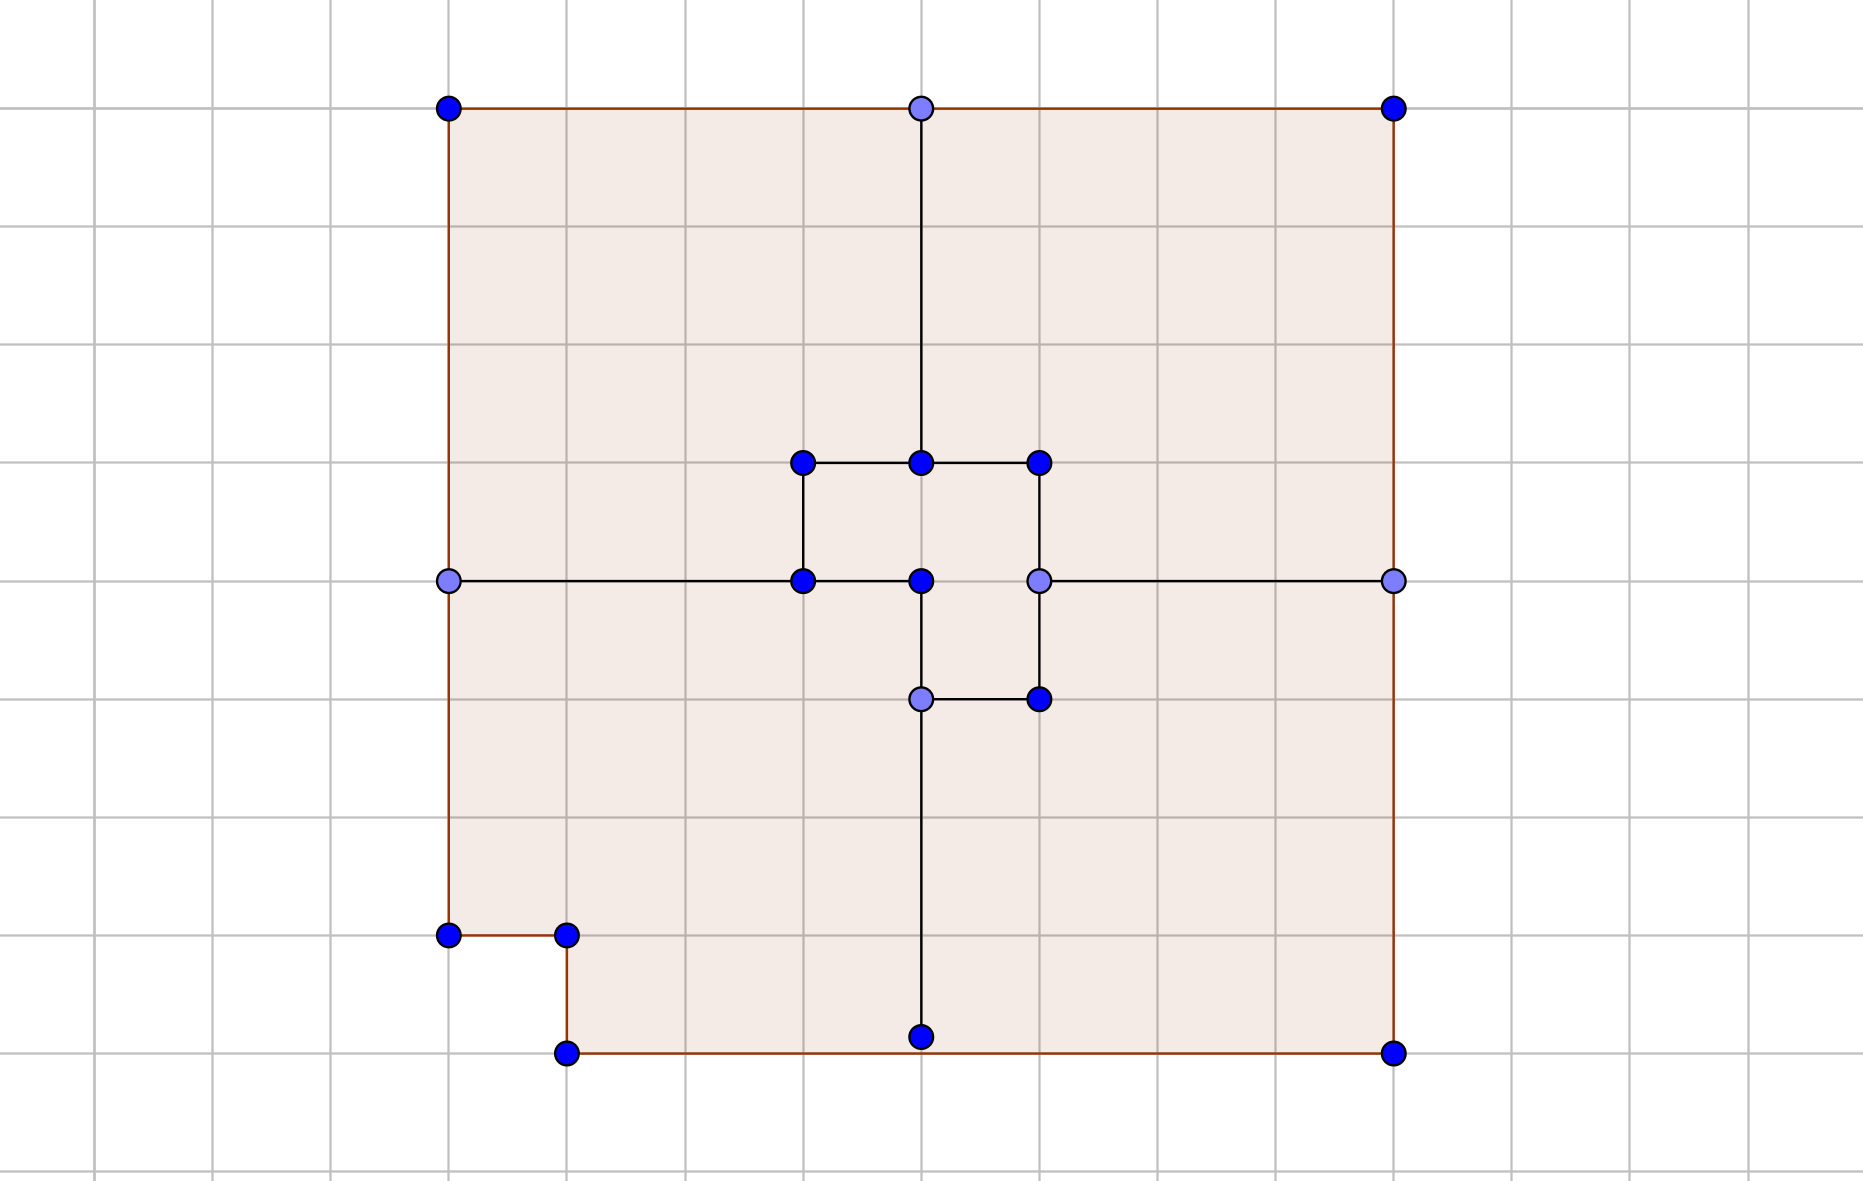
\includegraphics[width=\textwidth]{images/L-1}
\end{center}

We can divide the $2^{n+1}\times 2^{n+1}$ chessboard in the way shown above, so that the separate 5 parts of chessboard are 4 $2^n\times 2^n$ (with one corner unit removed) chessboard, and 1 \textit{L}-tile. It is obvious that \textit{L}-tile can be covered by one \textit{L}-tile, and according to inductive hypothesis, the 4 $2^n\times 2^n$ chessboard can be covered by certain number of \textit{L}-tiles too. Hence, the $2^{n+1}\times 2^{n+1}$ chessboard can be covered by \textit{L}-tiles. And we are done.

\qed

(b) \textbf{Proof:}\\

Similarly, we use induction to prove this as well.\\

\paragraph{Base step:} when $k=1$, the $2\times 2$ chessboard with a single square in the lower left corner deleted is still a \textit{L}-tile.\\

\paragraph{Inductive step:} Suppose when $k=n$, the $2^n\times 2^n$ chessboard can be covered by \textit{L}-tiles. We want to show when $k=n+1$, the $2^{n+1}\times 2^{n+1}$ chessboard can be covered by \textit{L}-tiles, too.\\

The strategy is that we find the midpoint of edges of this large square, connect the opposite two midpoints, separating the large square into 4 small squares each with edge length $2^n$.\\

Now we observe which part contains the deleted 1 unit of square. And we treat it as the deleted lower left corner in part (a). And similarly, we cut the large square into 5 parts as following:

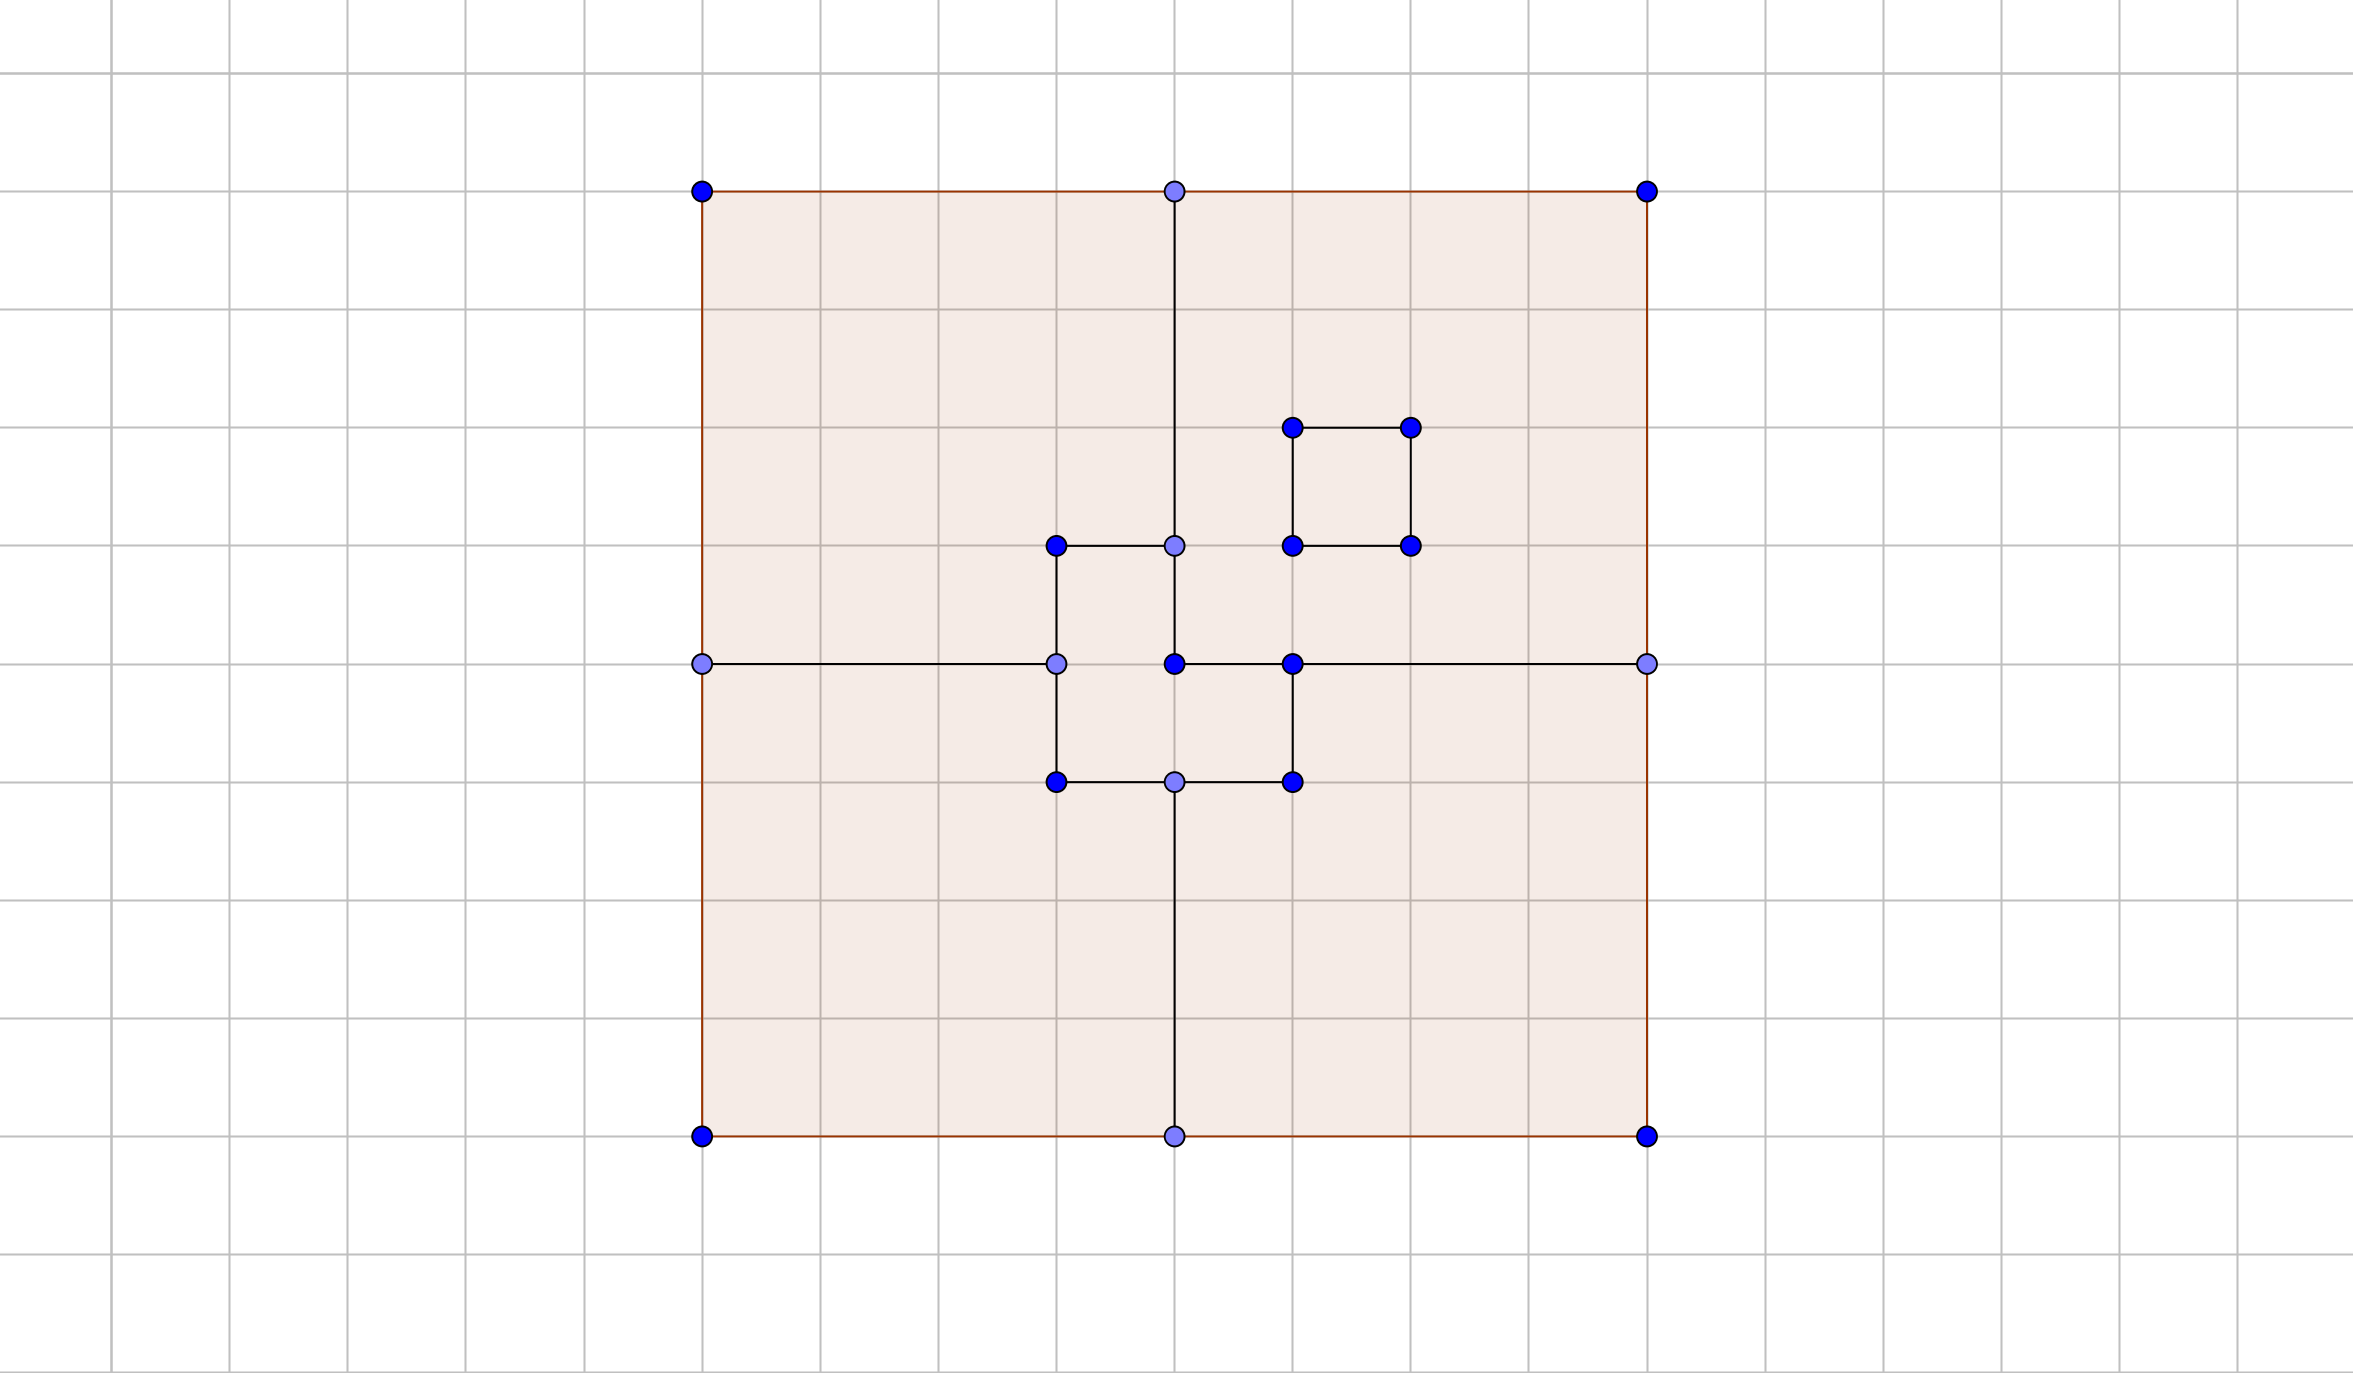
\includegraphics[width=\textwidth]{images/L-2}

So we have 1 \textit{L}-tile part, 3 $2^n\times 2^n$ chessboards missing a corner square, and a $2^n\times 2^n$ chessboard missing a random square inside it. Again, by inductive hypothesis, the $2^n\times 2^n$ chessboards (missing one square) can be covered by \textit{L}-tile, and the \textit{L}-tile can be covered by an \textit{L}-tile directly.\\

Hence a $2^k\times 2^k$ chessboard with \textit{any} single square deleted admits an \textit{L}-tiling, for any $k\in\mathbb{N}, k > 0.$

\qed

\end{homeworkProblem}

\end{document}
